%%%%%%%%%%%%%%%%%%%%%%% file template.tex %%%%%%%%%%%%%%%%%%%%%%%%%
%
% This is a general template file for the LaTeX package SVJour3
% for Springer journals.          Springer Heidelberg 2010/09/16
%
% Copy it to a new file with a new name and use it as the basis
% for your article. Delete % signs as needed.
%
% This template includes a few options for different layouts and
% content for various journals. Please consult a previous issue of
% your journal as needed.
%
%%%%%%%%%%%%%%%%%%%%%%%%%%%%%%%%%%%%%%%%%%%%%%%%%%%%%%%%%%%%%%%%%%%
%
% First comes an example EPS file -- just ignore it and
% proceed on the \documentclass line
% your LaTeX will extract the file if required
\begin{filecontents*}{example.eps}
%!PS-Adobe-3.0 EPSF-3.0
%%BoundingBox: 19 19 221 221
%%CreationDate: Mon Sep 29 1997
%%Creator: programmed by hand (JK)
%%EndComments
gsave
newpath
  20 20 moveto
  20 220 lineto
  220 220 lineto
  220 20 lineto
closepath
2 setlinewidth
gsave
  .4 setgray fill
grestore
stroke
grestore
\end{filecontents*}
%
\RequirePackage{fix-cm}
%
%\documentclass{svjour3}                     % onecolumn (standard format)
%\documentclass[smallcondensed]{svjour3}     % onecolumn (ditto)
\documentclass[smallextended]{svjour3}       % onecolumn (second format)
%\documentclass[twocolumn]{svjour3}          % twocolumn
%
\smartqed  % flush right qed marks, e.g. at end of proof
%
\usepackage{graphicx}
%
% \usepackage{mathptmx}      % use Times fonts if available on your TeX system
%
% insert here the call for the packages your document requires
%\usepackage{latexsym}
% etc.
%
% please place your own definitions here and don't use \def but
% \newcommand{}{}
%
% Insert the name of "your journal" with
% \journalname{myjournal}
%
\begin{document}

\title{Insert your title here%\thanks{Grants or other notes
%about the article that should go on the front page should be
%placed here. General acknowledgments should be placed at the end of the article.}
}
\subtitle{Do you have a subtitle?\\ If so, write it here}

%\titlerunning{Short form of title}        % if too long for running head

\author{First Author         \and
        Second Author %etc.
}

%\authorrunning{Short form of author list} % if too long for running head

\institute{F. Author \at
              first address \\
              Tel.: +123-45-678910\\
              Fax: +123-45-678910\\
              \email{fauthor@example.com}           %  \\
%             \emph{Present address:} of F. Author  %  if needed
           \and
           S. Author \at
              second address
}

\date{Received: date / Accepted: date}
% The correct dates will be entered by the editor


\maketitle

\begin{abstract}
Insert your abstract here. Include keywords, PACS and mathematical
subject classification numbers as needed.
\keywords{First keyword \and Second keyword \and More}
% \PACS{PACS code1 \and PACS code2 \and more}
% \subclass{MSC code1 \and MSC code2 \and more}
\end{abstract}

\section{Introduction}
\label{intro}
Your text comes here. Separate text sections with
\section{Section title}
\label{sec:1}
Text with citations \cite{RefB} and \cite{RefJ}.
\subsection{Subsection title}
\label{sec:2}
as required. Don't forget to give each section
and subsection a unique label (see Sect.~\ref{sec:1}).
\paragraph{Paragraph headings} Use paragraph headings as needed.
\begin{equation}
a^2+b^2=c^2
\end{equation}

\section{Image Labeling}

Part of the dataset is manually annotated to provide ground truth tip locations, leaf segmentation results and leaf consistency overtime. 
Tip locations are saved in TXT file \textcolor{red}{(TBD)}.
Leaf segmentation results are stored in PNG images with one color for each leaf.
The same color is used to represent the same leaf over a sequence of frames. 

We use RGB images for labeling because of better visualization. 
All plants are cropped out from the background and saved as JPG files. 
For Arabidopsis images, we label four frames each day. 
While for bean images, we label seven frames each day because of faster leaf movement. 
We develop a Matlab GUI interface for leaf labeling, as shown in Fig~\ref{fig:label}.
A user can open an image to label the two tips and annotate each leaf. 
The results will be automatically saved once a user goes to label the next image. 
This GUI is used to annotate leaves in each frame. 
For consistent annotation of the same leaf over time, we use the labeled results of each frame to find the correspondence according to leaf centers. 
Incorrect correspondence will be manually corrected. 

\begin{figure}[h]
\centering
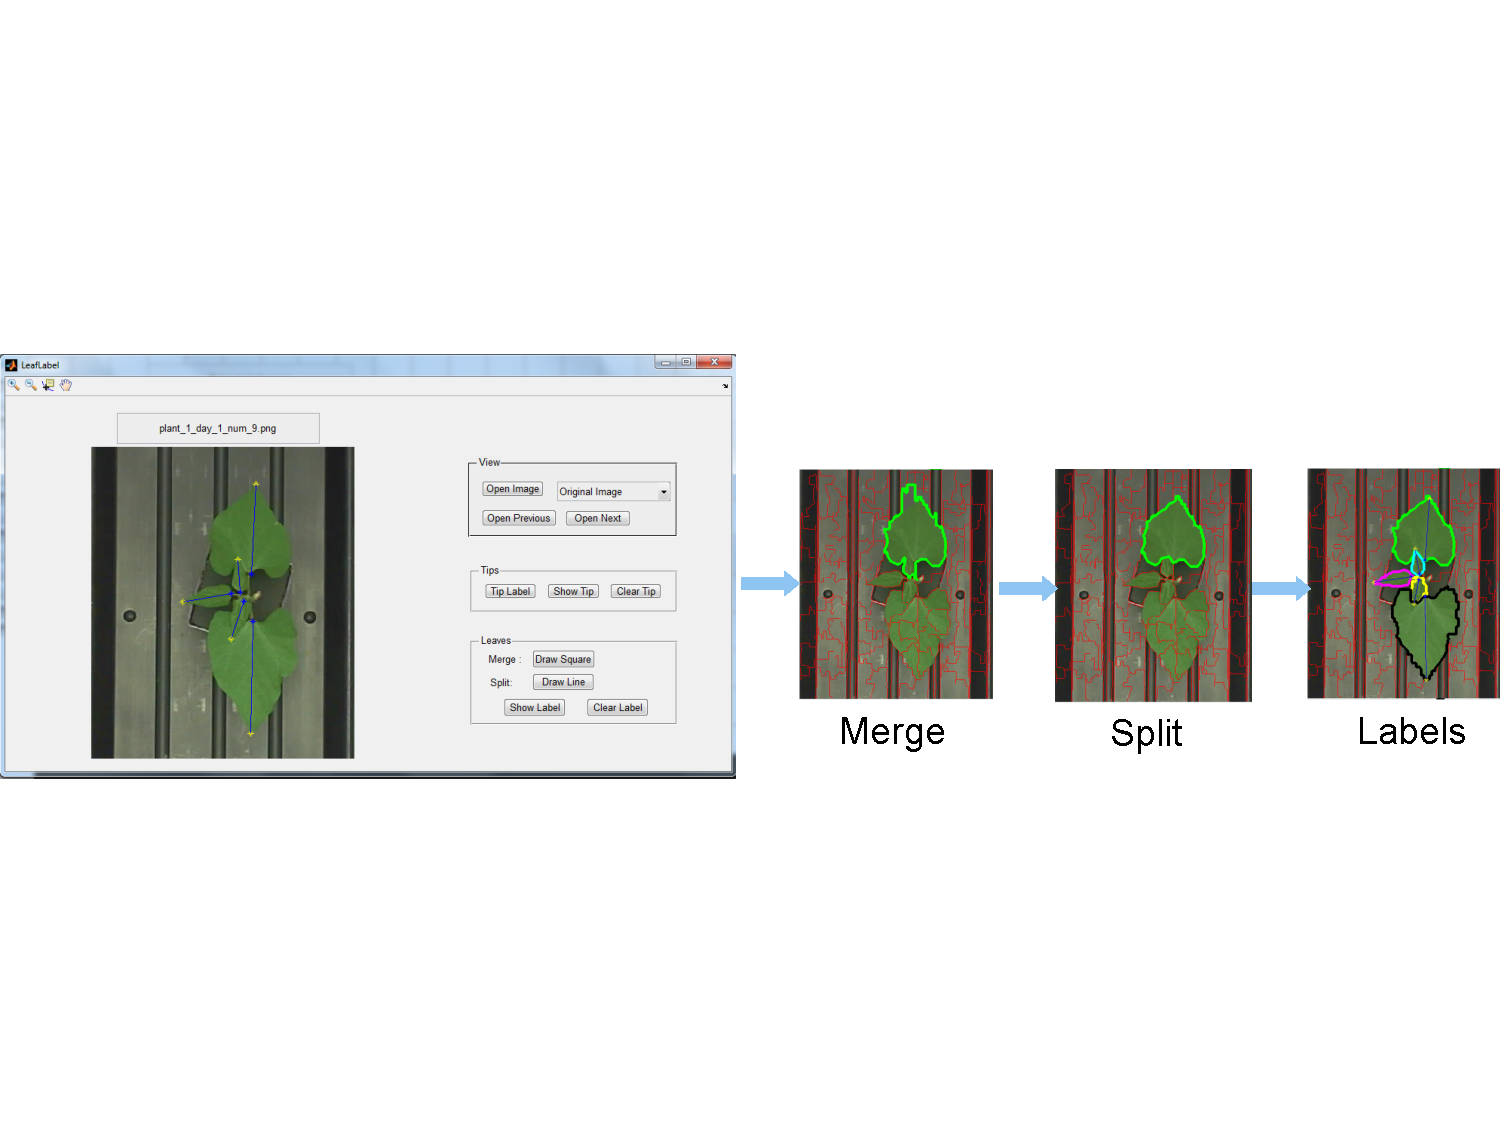
\includegraphics[width=.98\textwidth]{figure/labeling}\\
\caption{Leaf labeling process, including tip labels and leaf annotation.}
\label{fig:label}
\end{figure}

Tip label is implemented by clicking pairs of points on the image. 
The outer tip is always clicked before the inner tip. 
A line connecting each pair of tips will be shown immediately for visualization. 
Inaccurate labels can be deleted and relabeled. 

For leaf annotation, we use the idea of merging and splitting super pixels. 
There are six different numbers of super pixels: $100$, $200$, $300$, $500$, $800$, $1000$. 
The user can specify which level to use depending on how well the super pixels can separate the leaves from the background. 
Because one leaf can be covered by several super pixels and one super pixel can across two leaves or the foreground and background. 
We allow merging and splitting super pixels. 
Merging is implemented by drawing a rectangle on the image. 
Every super pixel overlapping with this rectangle will be merged together. 
Splitting is implemented by drawing a line separating a leaf from the background or from another leaf. 

As shown in Fig.~\ref{fig:label}, several super pixels that covers one leaf are first merged together to form a large super pixel. 
Since the top part of the super pixel covers some of the background and the bottom part covers another small leaf, two lines are drawn on this super pixel to split it. 
The leaf boundary is overlaid on the image for better visualization to guide the next action. 
This process continues until all leaves have been annotated. 

















% For one-column wide figures use
%\begin{figure}
%% Use the relevant command to insert your figure file.
%% For example, with the graphicx package use
%  
\includegraphics{example.eps}
%% figure caption is below the figure
%\caption{Please write your figure caption here}
%\label{fig:1}       % Give a unique label
%\end{figure}
%
%% For two-column wide figures use
%\begin{figure*}
%% Use the relevant command to insert your figure file.
%% For example, with the graphicx package use
%  
\includegraphics[width=0.75\textwidth]{example.eps}
%% figure caption is below the figure
%\caption{Please write your figure caption here}
%\label{fig:2}       % Give a unique label
%\end{figure*}
%
% For tables use
\begin{table}
% table caption is above the table
\caption{Please write your table caption here}
\label{tab:1}       % Give a unique label
% For LaTeX tables use
\begin{tabular}{lll}
\hline\noalign{\smallskip}
first & second & third  \\
\noalign{\smallskip}\hline\noalign{\smallskip}
number & number & number \\
number & number & number \\
\noalign{\smallskip}\hline
\end{tabular}
\end{table}


%\begin{acknowledgements}
%If you'd like to thank anyone, place your comments here
%and remove the percent signs.
%\end{acknowledgements}

% BibTeX users please use one of
%\bibliographystyle{spbasic}      % basic style, author-year citations
%\bibliographystyle{spmpsci}      % mathematics and physical sciences
%\bibliographystyle{spphys}       % APS-like style for physics
%\bibliography{}   % name your BibTeX data base

% Non-BibTeX users please use
\begin{thebibliography}{}
%
% and use \bibitem to create references. Consult the Instructions
% for authors for reference list style.
%
\bibitem{RefJ}
% Format for Journal Reference
Author, Article title, Journal, Volume, page numbers (year)
% Format for books
\bibitem{RefB}
Author, Book title, page numbers. Publisher, place (year)
% etc
\end{thebibliography}

\end{document}
% end of file template.tex

